% Name: Wavelength and amplitude
% Description: A sine wave along x with one wavelength λ marked from crest to crest, the amplitude A from the axis to a crest, and a crest and a trough labeled.
% Tags: wave, wavelength, amplitude, sine wave

\usetikzlibrary{arrows.meta}

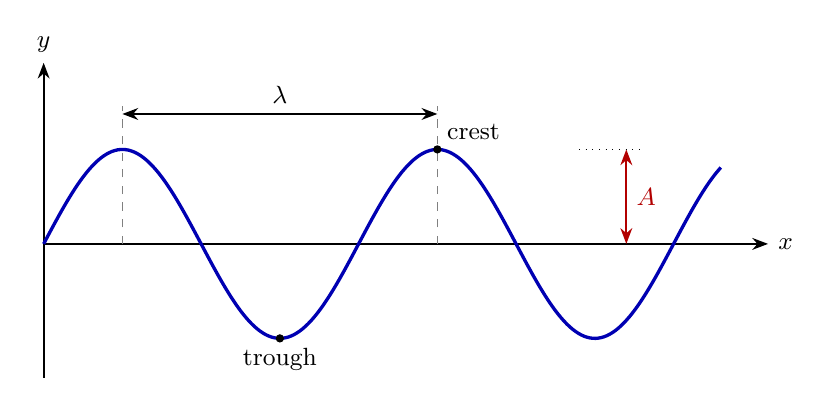
\begin{tikzpicture}[>={Stealth[length=2mm]}, every node/.style={font=\small}]
  % y = 1.2 sin(2 pi x / 4): crests at x = 1 and 5, a trough at x = 3.
  \draw[->, thick] (0,0) -- (9.2,0) node[right] {$x$};
  \draw[->, thick] (0,-1.7) -- (0,2.3) node[above] {$y$};
  \draw[very thick, blue!70!black, domain=0:8.6, samples=120, smooth] plot (\x, {1.2*sin(90*\x)});
  \draw[dashed, gray] (1,0) -- (1,1.75) (5,0) -- (5,1.75);
  \draw[<->, thick] (1,1.65) -- node[above] {$\lambda$} (5,1.65);
  \draw[<->, thick, red!70!black] (7.4,0) -- node[right] {$A$} (7.4,1.2);
  \draw[dotted] (6.8,1.2) -- (7.6,1.2);
  \node[above right] at (5,1.2) {crest};
  \node[below] at (3,-1.2) {trough};
  \fill (5,1.2) circle (1.5pt) (3,-1.2) circle (1.5pt);
\end{tikzpicture}
